%%%%%%%%%%%%%%%%%%%%%%%%%%%%%%%%%%%%%%%%%
% Tecnologico de Costa Rica/Instructivo de Laboratorio de Electricidad I
% LaTeX Template
% Version 3.1 (25/3/14)
%
% This template has been downloaded from:
% http://www.LaTeXTemplates.com
%
% Original author:
% Linux and Unix Users Group at Virginia Tech Wiki 
% (https://vtluug.org/wiki/Example_LaTeX_chem_lab_report)
%
% License:
% CC BY-NC-SA 3.0 (http://creativecommons.org/licenses/by-nc-sa/3.0/)
%
%%%%%%%%%%%%%%%%%%%%%%%%%%%%%%%%%%%%%%%%%

%----------------------------------------------------------------------------------------
%	PACKAGES AND DOCUMENT CONFIGURATIONS
%----------------------------------------------------------------------------------------

\documentclass{report}
\usepackage{url}
\usepackage{float}
\usepackage[utf8]{inputenc}
\usepackage[spanish,activeacute]{babel} %Permite la escritura intiutiva en español
\usepackage[version=3]{mhchem} % Package for chemical equation typesetting
\usepackage{siunitx} % Provides the \SI{}{} and \si{} command for typesetting SI units
\usepackage{graphicx} % Required for the inclusion of images
\usepackage[siunitx]{circuitikz} %Este se usa para hacer circuitos
%\usepackage{natbib} % Required to change bibliography style to APA
\usepackage{amsmath} % Required for some math elements 
\usepackage{array}
\usepackage{hyperref}
\hypersetup{
    colorlinks=true,
    linkcolor=blue,
    filecolor=magenta,      
    urlcolor=blue,
    citecolor=blue,
    bookmarks=true,
    pdfpagemode=FullScreen,
}
\setlength\parindent{0pt} % Removes all indentation from paragraphs

\renewcommand{\labelenumi}{\alph{enumi}.} % Make numbering in the enumerate environment by letter rather than number (e.g. section 6)
\usepackage{fancyhdr}
\pagestyle{fancy}
\lhead{Instructivo de Laboratorio de Electricidad I}
\rhead{\begin{picture}(0,0) \put(-60,0){
\includegraphics[width=20mm]{logo}} \end{picture}}

%\usepackage{times} % Uncomment to use the Times New Roman font
\newcommand{\obj}{Objetivos}
\newcommand{\inv}{Investigación previa}
\newcommand{\mat}{Materiales y equipo}
\newcommand{\pro}{Procedimiento}
\newcommand{\capacidad}{Al finalizar este laboratorio el estudiante estará en capacidad de:}
\newcommand{\antesde}{Antes de empezar el laboratorio presente el siguiente cuestionario lleno.}
%----------------------------------------------------------------------------------------
%	DOCUMENT INFORMATION
%----------------------------------------------------------------------------------------

\addto\captionsspanish{\renewcommand{\chaptername}{Laboratorio}}
\addto\captionsspanish{\renewcommand{\tablename}{Tabla}}
\begin{document}


\begin{titlepage}

\begin{center}
\vspace*{-1in}
\begin{figure}[htb]
\begin{center}

\includegraphics[width=11cm]{logo}
\end{center}
\end{figure}
\vspace*{0.4in}
\begin{Large}
ESCUELA DE INGENIERIA ELECTROMECANICA\\
\vspace*{0.15in}
AREA ELECTRICA\\
\vspace*{0.8in}
\end{Large}
\vspace*{0.2in}
\begin{Large}
\textbf{MANUAL DE PRACTICAS DE LABORATORIO} \\
\end{Large}
\vspace*{0.3in}
\begin{large}
LABORATORIO DE ELECTRICIDAD I\\
\end{large}
\vspace*{2.5in}
\begin{Large}
\textbf{\today}\\
Versión: 1.1\\
\end{Large}
\rule{80mm}{0.1mm}\\
\vspace*{0.1in}
\begin{large}
Realizado por: Lisandro Araya \\
Juan J. Rojas y Nicolas Vaquerano\\
\end{large}
\end{center}

\end{titlepage}

\tableofcontents

\chapter{Empleo y lectura de instrumentos de medición eléctrica para corriente y voltaje}
\section{\obj}
Al finalizar la práctica de laboratorio el estudiante estará en capacidad de:
\begin{itemize}
\item Comprender las limitaciones de lectura en los voltímetros y amperímetros de corriente continua en varias escalas.
\item Calcular la resistencia equivalente de un elemento utilizando el método indirecto de la Ley de Ohm.
\item	Comprobar experimentalmente la Ley de Ohm.
\item	Demostrar el concepto de linealidad en una resistencia.
\end{itemize}

\section{\inv}
\antesde
\begin{enumerate}
\item	Defina el significado de voltaje, corriente y resistencia.
\item	¿Cómo se debe conectar un amperímetro para medir la corriente en una carga? ¿Qué pasa si no se conecta así, qué peligros puede haber?
\item	¿Cómo se debe conectar un voltímetro para medir el voltaje en una carga? ¿Qué pasa si no se conecta así, qué peligros puede haber?
\item	¿Cómo se define el porcentaje de error en la lectura de un instrumento analógico y uno digital?
\item	Según las especificaciones de su multímetro y para los distintos rangos de medición, defina cuál es el porcentaje de error en las lecturas de voltaje, corriente.
\item	¿Qué relación tienen entre si los términos eléctricos de potencia y energía?
\item	¿Qué es la resistencia interna en un voltímetro y amperímetro? ¿Cuál es el valor en cada caso?
\item	Investigue por qué la temperatura afecta la resistencia de un conductor.
\item	¿Qué significa la linealidad de un dispositivo eléctrico? ¿Qué consecuencias tiene esta?
\end{enumerate}

\section{\mat}
\begin{itemize}
\item 1 multímetro digital (a proveer por los estudiantes)
\item 1 Voltímetro analógico de CD
\item 1 Amperímetro analógico CD
\item 1 socket para bombillo incandescente
\item 1 bombillo incandescente
\item 1 resistencia de potencia de 500 $\Omega$ en 100 \si{W}
\item 10 cables conectores medianos
\item 1 fuente variable de voltaje DC
\end{itemize}

\section{\pro}
\begin{enumerate}
\item Realice las conexiones del circuito tal y como se indica en la Figura \ref{fig:L1F1}.
\begin{figure}[H]
\centering
\begin{circuitikz} \draw
(0,0) 	to[american voltage source, l=$\mathrm{V}_{fuente}$] (0,2)
		to[ammeter] (3,2) -- (3,1.9)
		to[lamp, l_=B, *-*] (3,0.1) -- (3,0) -- (0,0)
(3,1.9) -- (4,1.9)
		to[voltmeter] (4,0.1) -- (3,0.1)
		
;
\end{circuitikz}
\caption{Medición de corriente y voltaje en un circuito.}
\label{fig:L1F1}
\end{figure}

\item Encienda la fuente con un voltaje de 120 V y espere unos minutos mientras el bombillo se calienta. No se olvide de incluir en la discusión la razón por la cual se debe esperar que el bobillo caliente y si habrían cambiado los datos si se midieran en frío.
\item Una vez que el bombillo calentó mida la corriente que circula por el bombillo y el voltaje que cae en este, anote el resultado en la Tabla \ref{tab:L1T1}, para las mediciones utilice instrumentos analógicos. Calcule indirectamente el valor de la resistencia interna del bombillo.
\item	Repita las mediciones utilizando los valores de voltaje que indica la Tabla \ref{fig:L1F1} y complete la misma. Calcule indirectamente para cada caso el valor de la resistencia interna del bombillo.
\item	Grafique el comportamiento de la resistencia interna del bombillo y analice el comportamiento. ¿Es lineal? ¿Por qué? 
\item	Cambie ahora el bombillo por una resistencia de potencia de 500$\Omega$/100\si{W}, repita los pasos anteriores empezando con cero voltios en la fuente, llene la Tabla \ref{tab:L1T2}, para las mediciones utilice instrumentos analógicos. Calcule indirectamente el valor de la resistencia.
\emph{Nota: En este caso no es necesario dejar la resistencia calentando.}
\item	Grafique el comportamiento de la resistencia. Compruebe la validez de la ley de Ohm. Analice el comportamiento. ¿Es lineal? ¿Por qué?
\item	Repita esta última medición (Tabla \ref{tab:L1T2}) con un multímetro digital (usandolo como amperimetro), ¿cómo cambia la medición y el error de esta?
\end{enumerate}

\begin{table}[H]
	\caption{Valores experimentales de corriente y voltaje del bombillo}
	\label{tab:L1T1}
	\centering
	\begin{tabular}[t]{| >{\centering\arraybackslash}m{2cm} | >{\centering\arraybackslash}m{2cm} |
	>{\centering\arraybackslash}m{2cm} |}
		\hline
		$V_B$ (\si{V}) & $I_B$(\si{\milli\ampere}) & $R_B$($\Omega$)\\
		\hline
		0 & & \\
		\hline
		5 & & \\
		\hline
		10 & & \\
		\hline
		15 & & \\
		\hline				
		20 & & \\
		\hline
		30 & & \\
		\hline		
		40 & & \\
		\hline
		60 & & \\
		\hline
		80 & & \\
		\hline	
		100 & & \\
		\hline
		120 & & \\
		\hline	
	\end{tabular}
\end{table}
\begin{table}[H]
	\caption{Valores experimentales de corriente y voltaje en la resistencia}
	\label{tab:L1T2}
	\centering
	\begin{tabular}[t]{| >{\centering\arraybackslash}m{2cm} | >{\centering\arraybackslash}m{2cm} |
	>{\centering\arraybackslash}m{2cm} |}
		\hline
		$V_R$ (\si{V}) & $I_R$(\si{\milli\ampere}) & R($\Omega$)\\
		\hline
		0 & & \\
		\hline
		5 & & \\
		\hline
		10 & & \\
		\hline
		15 & & \\
		\hline				
		20 & & \\
		\hline
		30 & & \\
		\hline		
		40 & & \\
		\hline
		60 & & \\
		\hline
		80 & & \\
		\hline	
		100 & & \\
		\hline
		120 & & \\
		\hline	
	\end{tabular}
\end{table}

\chapter{Resistencia y resistividad}
\section{\obj}
Al finalizar la práctica de laboratorio el estudiante estará en capacidad de:
\begin{itemize}
\item Verificar cómo influye la longitud y el área transversal de un conductor eléctrico, en la resistencia del mismo.
\item	Comprobar que el valor de resistividad solo depende del tipo de material y no de su longitud o área transversal.
\item	Utilizar el ohmímetro para medir diversos valores de resistencia y comparar los datos con sus magnitudes nominales.
\end{itemize}
\section{\inv}
\antesde
\begin{enumerate}
\item	Liste el código de colores utilizado para definir el valor de resistencia y su tolerancia.
\item	Investigue sobre los distintos materiales y técnicas empleadas en la fabricación de resistencias.
\item Liste los valores comerciales más comunes para resistencias de $\frac{1}{2}$ \si{\watt}.
\item	¿Cuál es la resistencia mínima capaz de medir el multímetro empleado y cómo incide ésta en las lecturas de muy baja y de alta impedancia?
\item	¿Qué significan los conceptos de resistividad y conductividad? ¿Cómo se diferencian de resistencia y conductancia?
\item	¿Cómo afecta la frecuencia la capacidad de conducción de un metal?
\item	Investigue sobre la conductividad eléctrica del agua destilada. ¿Es un medio conductor o aislante?
\item	Liste la resistividad eléctrica del oro, cobre, hierro, plomo, estaño, zinc y nicromo. Compare éstos datos con sus respectivas conductividades. ¿Analice qué relación existe entre ambos parámetros?
\item	Investigue que es un dieléctrico y describa las características de cinco tipos distintos. ¿Por qué la forma constructiva incide en la capacidad de aislamiento?
\item	¿En qué unidades se mide el calibre de los conductores eléctricos?
\item	¿En qué consiste el proceso de galvanizado del hierro y cuál es su función? Investigue cómo afecta este proceso a la capacidad de conducción del hierro.
\item	Describa las propiedades eléctricas del óxido de hierro.
\item	Investigue por qué no hay que tocar ambas puntas con las manos cuando se mide una resistencia eléctrica ¿Esta restricción es válida para altos o bajos valores de resistencia? Explique.
\item	¿Cuál es la diferencia que existe entre un ohmímetro, un mili ohmímetro y un mega ohmímetro? Investigue qué otro nombre comercial tiene este último.
\end{enumerate}
\section{\mat}
\begin{itemize}
\item	1 multímetro digital (a proveer por el grupo)
\item	1 Mili ohmímetro digital
\item	6 Tablas de alambre de diversos materiales
\item	Cables conectores pequeños y medianos
\item	5 resistencias de 1 watt de distintos valores
\end{itemize}
\section{\pro}
\subsection{Resistividad}
\begin{enumerate}
\item	Utilizando alambres de diferentes materiales, según se indica, proceda a medir la resistencia para cada uno de los diámetros y longitudes indicadas, utilizando para ello el mili ohmímetro.
\item	Para diámetros de igual material, se debe medir el valor de la resistencia para longitudes de 1 m, 2 m, 3 m, 4 m, 5 m y 10 m. Anote los resultados en la Tabla \ref{tab:L2T1}.
\begin{table}[H]
	\caption{Valores de resistencia de diversos materiales según longitud y área transversal}
	\label{tab:L2T1}
	\centering
	\begin{tabular}[h]{|>{\centering\arraybackslash}m{2cm}|>{\centering\arraybackslash}m{2cm} |c|c|c|c|c|c|}
		\cline{3-8}
		\multicolumn{2}{c|}{}&\multicolumn{6}{c|}{Resistencia ($\Omega$)}\\
		\hline
		Material & Diametro (mm) & 1m & 2m & 3m & 4m & 5m & 10m\\
		\hline
		Nicromo & 0.72 & & & & & &\\
		\hline
		Nicromo & 1.00 & & & & & &\\
		\hline
		Hierro Galvanizado & 0.75 & & & & & &\\
		\hline
		Hierro Galvanizado & 1.19 & & & & & &\\
		\hline
		Cobre & 0.77 & & & & & &\\
		\hline
		Cobre & 1.19 & & & & & &\\
		\hline
	\end{tabular}
\end{table}
\item Calcule los valores de la constante del conductor como un promedio de los valores que se obtuvieron, para cada uno de los materiales. Anote sus cálculos en la  Tabla \ref{tab:L2T2}.
\begin{table}[H]
	\caption{Valores de resistividad de diversos materiales}
	\label{tab:L2T2}
	\centering
	\begin{tabular}[h]{|>{\centering\arraybackslash}m{2cm}|>{\centering\arraybackslash}m{2cm} |c|c|c|c|c|c|c|}
		\cline{3-9}
		\multicolumn{2}{c|}{}&\multicolumn{7}{c|}{Resistividad ($\Omega\si{m}$)}\\
		\hline
		Material & Diametro (mm) & 1m & 2m & 3m & 4m & 5m & 10m & Promedio\\
		\hline
		Nicromo & 0.72 & & & & & & & \\
		\hline
		Nicromo & 1.00 & & & & & & & \\
		\hline
		Hierro Galvanizado & 0.75 & & & & & & & \\
		\hline
		Hierro Galvanizado & 1.19 & & & & & & & \\
		\hline
		Cobre & 0.77 & & & & & & & \\
		\hline
		Cobre & 1.19 & & & & & & & \\
		\hline
	\end{tabular}
\end{table}
\item Por medio de métodos estadísticos demuestre que la resistividad es constante para cada material y es independiente de la longitud o del área transversal.
\item Demuestre que la resistencia es proporcional a la distancia e inversamente proporcional al área transversal.
\end{enumerate}
\subsection{Resistencia}
\begin{enumerate}
\item	Encontrará en la mesa 5 resistencias de 1 watt, lea el valor de cada una de ellas utilizando el código de colores y confirme sus magnitudes con el multímetro. En cada caso, tabule las tolerancias definidas en ellas y el porcentaje de error propio del medidor para los rangos empleados.
\item	Explique por qué cambia la lectura en el multímetro al tocar con sus manos los extremos de una resistencia de alta impedancia.
\end{enumerate}

\chapter{Circuitos en serie y paralelo}
\section{\obj}
\capacidad
\begin{itemize}
\item	Verificar las características eléctricas de los circuitos en serie y en paralelo.
\item	Realizar conexiones eléctricas de circuitos con configuraciones en serie y en paralelo.
\item	Calibrar una resistencia variable de acuerdo al valor requerido
\end{itemize}

\section{\inv}
\antesde
\begin{enumerate}
\item	¿Cómo se calcula el valor equivalente de varias resistencias en paralelo?
\item	¿Cómo se calcula el valor equivalente de varias resistencias en serie?
\item	¿Qué es un divisor de tensión? ¿Cómo se calcula? ¿Para qué tipo de configuraciones sirve?
\item	¿Qué es un divisor de corriente? ¿Cómo se calcula? ¿Para qué tipo de configuraciones sirve?
\item	¿Qué son las leyes de Kirchhoff? ¿Qué dicen cada una de ellas? ¿Cuál es su utilidad?
\item	¿Qué es un valor nominal de un dispositivo? Cuando se calcula los valores teóricos ¿se deben utilizar siempre los valores nominales de los dispositivos?
\item	¿Qué es un potenciómetro? ¿Cuáles son sus aplicaciones? ¿En qué se diferencia con una resistencia variable? ¿Se puede utilizar un potenciómetro como resistencia variable y de ser así cómo sería?
\item	Resuelva teóricamente el laboratorio para los valores nominales de los dispositivos, para ello utilice por aparte tanto la ley de Ohm, leyes de Kirchhoff y también las reglas de división de voltaje y corriente donde corresponda
\end{enumerate}

\section{\mat}
\begin{itemize}
\item	1 multímetro digital (a proveer por el grupo)
\item	3 resistencias variables de 1 k\si{\ohm}
\item	Cables conectores pequeños
\end{itemize}

\section{\pro}
\subsection{Circuitos en serie}
\begin{enumerate}
\item	Coloque en cada uno de los potenciómetros el valor solicitado según la Figura \ref{fig:L3F1}.

\begin{figure}[H]
\centering
\begin{circuitikz} \draw
(0,0) 	to[american voltage source, l=30\si{\volt}] (0,2)
		to[resistor, l=600\si{\ohm}] (2,2)
		to[resistor, l=400\si{\ohm}] (4,2)
		to[resistor, l=240\si{\ohm}] (6,2) -- (6,0)
		-- (0,0)
				
;
\end{circuitikz}
\caption{Circuito serie.}
\label{fig:L3F1}
\end{figure}

\item	Arme el circuito de la figura 1 sin la fuente de voltaje; utilizado un ohmímetro mida la resistencia equivalente que vería la fuente y compárela con la calculada anteriormente.
\item	Siguiendo el protocolo adecuado añada la fuente del voltaje al circuito.
\item	Tome la lectura de la corriente que fluye en cada uno de los elementos, el voltaje que cae en cada elemento; tabúlelo adecuadamente.
\item	Utilizado los valores reales de los dispositivos, calcule todos los valores teóricos de los voltajes y corrientes de los elementos del circuito; compruebe con ellos la validez de las leyes de Kirchhoff y la regla de división de voltaje o corriente según corresponda.
\end{enumerate}

\subsection{Circuitos en paralelos}
\begin{enumerate}
\item	Revise cada uno de los potenciómetros para comprobar el valor solicitado según la Figura \ref{fig:L3F2}. , tenga cuidado con ello.

\begin{figure}[H]
\centering
\begin{circuitikz} \draw
(0,0) 	to[american voltage source, l=30\si{\volt}] (0,2) -- (1,2)
		to[resistor, l=600\si{\ohm}, *-*] (1,0)
		(1,0) -- (3,0)
		(1,2) -- (3,2)
		to[resistor, l=400\si{\ohm}, *-*] (3,0)
		(3,0) -- (5,0)
		(3,2) -- (5,2)
		to[resistor, l=240\si{\ohm}] (5,0)
		(0,0) -- (1,0)
				
;
\end{circuitikz}
\caption{Circuito paralelo.}
\label{fig:L3F2}
\end{figure}

\item	Arme el circuito de la Figura \ref{fig:L3F2}. sin la fuente de voltaje; utilizado un ohmímetro mida la resistencia equivalente que vería la fuente y compárela con la calculada anteriormente.
\item	Siguiendo el protocolo adecuado añada la fuente del voltaje al circuito, luego tome la lectura de la corriente que fluye en cada uno de los elementos, el voltaje que cae en cada elemento; tabúlelo adecuadamente.
\end{enumerate}

\chapter{Taller de simulación de circuitos}
\section{\obj}
\capacidad
\begin{itemize}
\item	Instalar un software de simulación por computadora enfocando su uso a circuitos de corriente directa, tanto con fuentes dependientes como independientes.
\item	Comprender el efecto del cambio de magnitud en un elemento sobre el resto de un sistema eléctrico.
\item	Simular circuitos eléctricos en un programa adecuado.
\end{itemize}
\section{\inv}
\antesde
\begin{enumerate}
\item	Averigüe cómo conseguir los programas de simulación de circuitos PSIPCE, Multisim o TINA.¿Dónde se consiguen en línea? ¿Cuáles son las compañías que los producen? ¿Cómo se bajan, cuál es su costo, en cuáles plataformas y dispositivos trabajan? ¿Compare sus ventajas y desventajas? ¿Con qué tipo de archivo de datos trabajan y si estos son compatibles entre programas? Siéntase en libertad de añadir otros programas de simulación.
\item	Escoja uno de ellos para trabajar, indique y explique las razones que lo motivaron en su elección.
\item	Redacte un resumen ejecutivo de cómo se usa el programa escogido para dibujar el circuito, añadir componentes, simular el problema y mostrar los resultados, para circuitos con resistencias, fuentes de voltaje y corriente tanto dependientes como independientes.
\item	Lleve simulado el circuito de la Figura \ref{fig:L4F1} de este taller.
\end{enumerate}
\section{\mat}
\begin{itemize}
\item 1 equipo de cómputo adecuado para realizar el taller (Laptop, notebook, Tablet, Smartphone); este equipo debe tener previamente cargado el simulador a utilizar.
\end{itemize}
\section{\pro}
Este taller será realizado en parejas, escoja un compañero de trabajo y realice lo siguiente:
\begin{enumerate}
\item	Presente al profesor el circuito simulado, en donde se muestre la potencia de la fuente de 3 V, la corriente en la fuente de 4 V y el voltaje en la resistencia de 6 \si{\ohm}; para cada uno de los siguientes valores de la resistencia R.

\begin{tabular}{p{4cm}p{4cm}}
\textbullet{Un corto} & \textbullet{Un abierto} \\
\textbullet{1 \si{\ohm}} & \textbullet{10 \si{\ohm}}
\end{tabular}


\begin{figure}[H]
\centering
\begin{circuitikz}[scale=1.1] \draw
(0,0) 	to[american voltage source, l=3\si{\volt}] (0,2)
		to[resistor, l=2\si{\ohm}] (2,2) -- (6,2)
		to[resistor, l_=5\si{\ohm}, *-*] (6,0) 
		to[resistor, l_=2\si{\ohm}, *-*] (4,0)
		to[resistor, l=1\si{\ohm}, *-*] (4,2)
(0,0)   to[resistor, l=4\si{\ohm},i<_=$I_x$] (2,0)
		to[american current source, l={0,2}\si{\ampere}, *-*] (2,2)
(4,0)	to[american voltage source, l_=5\si{\volt}] (2,0)
(6,2)	to[american controlled current source, l=$I_x$] (8,2)
		to[resistor, l_=1\si{\ohm},*-*] (8,0)
		to[resistor, l_=3\si{\ohm}] (6,0)
(8,2) 	to[resistor, l=3\si{\ohm}] (10,2) -- (10,-2) -- (8,-2)
		to[resistor, l_=R] (6,-2)
		to[resistor, l_=4\si{\ohm},*-] (4,-2)
(2,-2)	to[american voltage source, l=4\si{\volt},*-] (4,-2)
(6,-2) -- (6,0)
(0,0)	to[resistor, l=6\si{\ohm}] (0,-4)
(2,0)	-- (2,-4) -- (0,-4)
(2,-4) 	to[resistor, l=2\si{\ohm},*-*] (8,-4)
		to[resistor, l=5\si{\ohm}] (8,-2) -- (8,0)
(10,-2) to[short, *-] (10,-4) -- (8,-4)
;
\end{circuitikz}
\caption{Circuito paralelo.}
\label{fig:L3F2}
\end{figure}

\item	Simule los circuitos que el profesor le presentará, presentando los resultados solicitados.
\end{enumerate}

\chapter{Taller de implementación de un circuito en una
protoboard}

\section{\obj}
\capacidad
\begin{itemize}
\item Implementar en una protoboard un circuito mixto serie y paralelo.
\item Comprobar los valores simulados de un circuito eléctrico implementado en
una protoboard.
\end{itemize}
\section{\inv}
\antesde
\begin{enumerate}
\item ¿Qué es una protoboard? Investigue un poco sobre su historia ¿Qué tipos de
protoboards existen? ¿Quiénes son los fabricantes? ¿Dónde se pueden
comprar, cuánto cuestan?
\item ¿Cómo se implementa un circuito eléctrico en una protoboard? Algunas
protoboard tienen unas terminales tipo banana externas ¿están estas
conectadas al resto de la tableta? Si no es así ¿cómo se conectarían?
\item ¿Cuáles son las limitaciones del circuito a implementar en una protoboard en
cuanto a voltaje, corriente, potencia, dimensiones físicas, tamaño del circuito
y otras?
\item ¿Qué tipo de conectores eléctricos se utilizan al implementar un circuito en
una protoboard?
\item Investigue qué es una ferroboard, una tabla de wire wrap y un circuito
impreso, compare estos con las protoboard, en cuanto a ventajas,
aplicaciones, entre otros.
\item Lleve simulado el circuito a utilizar en este taller.
\end{enumerate}

\section{Consideraciones para la implementación del circuito}
\begin{itemize}
\item Utilice cable telefónico con diferentes colores de aislante, aproveche estos
para implementar algún tipo de código de colores para el alambrado (por
ejemplo, rojo para el positivo de la fuente de alimentación, cable negro para
el negativo de la fuente, verde para demás conexiones).
\item No pase un cable encima de otro, ni encima o debajo de un componente, ni
un componente encima de otro componente.
\item Trate de no hacer esquinas con el cable, utilice para ello los otros huecos del
nodo; si debe hacerlas trate de que el cable quede lo más recto posible.
\item No haga quiebres de 90\si{\degree} en los cables o dispositivos, estos se pueden romper.
\item No corte las patillas de los componentes, la protoboard se utiliza
para prototipos si corta las patillas de los elementos estos podrían no ser
útiles luego.
\item Trate de que los dispositivos iguales queden del mismo tamaño.
\end{itemize}

\section{Materiales y Equipo}
\begin{enumerate}
\item 1 Protoboard
Cable telefónico
\item 1 multímetro digital
\item Resistencias de $\frac{1}{2}$ \si{\watt}, valores de 1 \si{\kilo\ohm}; 1,2 \si{\kilo\ohm}; 2,2 \si{\kilo\ohm}; 3,3 \si{\kilo\ohm}; 5,6 \si{\kilo\ohm} y 6,8 \si{\kilo\ohm} (una de cada una).
\item Cables conectores pequeños (a proveer por la Escuela)
\item 1 fuente variable de voltaje DC (a proveer por la Escuela)
\end{enumerate}

\section{\pro}
\begin{enumerate}
\item Mida y tabule los valores reales de todos los elementos del circuito (esta tabla
será la número 1).
\item Implemente en una protoboard el circuito mostrado en la Figura \ref{fig:L5F1}. Tome en cuenta que se le evaluará la presentación
estética del mismo.
\begin{figure}[H]
\centering
\begin{circuitikz} [scale=1]\draw
(0,0) 	to[american voltage source, l=30\si{\volt}] (0,3)
		to[short,i>_=$i_T$] (1,3) node[below]{a}
		to[resistor, l={2,2}\si{\kilo\ohm},i>_=$i_2$, *-*] (4,3) node[above]{c}
		to[resistor, l={3,3}\si{\kilo\ohm},i>_=$i_3$, *-*] (7,3) node[right]{d} -- (7,0)
		to[resistor, l_={1,2}\si{\kilo\ohm}, *-] (0,0) node[left]{e}
(1,3)   -- (1,4.5)
		to[resistor, l={1}\si{\kilo\ohm},i>_=$i_1$] (4,4.5) node[above]{b}
		to[resistor, l={6,8}\si{\kilo\ohm}] (7,4.5) -- (7,3)
(4,3)   -- (4,1.5)
		to[resistor, l={5,6}\si{\kilo\ohm},i>_=$i_4$, -*] (7,1.5)
		
;
\end{circuitikz}
\caption{Circuito mixto serie-paralelo.}
\label{fig:L5F1}
\end{figure}

\item Solicítele al profesor que le revise su trabajo.
\item Una vez que tiene la aprobación del profesor mida las corrientes del circuito, tome como teóricas los valores simulados, tabule los valores en la Tabla \ref{tab:L5T1}.

\begin{table}[H]
	\caption{Corrientes del circuito mixto}
	\label{tab:L5T1}
	\centering
	\begin{tabular}[t]{| >{\centering\arraybackslash}m{2cm} | >{\centering\arraybackslash}m{2cm} |
	>{\centering\arraybackslash}m{2cm} | >{\centering\arraybackslash}m{2cm} |}
		\hline
		Variable & Teórico & Experimental & \% de error\\
		\hline
		$i_t$ & & & \\
		\hline
		$i_1$ & & & \\
		\hline
		$i_2$ & & & \\
		\hline
		$i_3$ & & & \\
		\hline				
		$i_4$ & & & \\
		\hline
		$i_1 + i_2$ & & & \\
		\hline		
		$i_3 + i_4$ & & & \\
		\hline
		$i_1 + i_3 + i_4$ & & & \\
		\hline
		$i_{1,2\si{\kilo\ohm}}$ & & & \\
		\hline			
	\end{tabular}
\end{table}

\item Mida ahora los voltajes del circuito, tome como teóricas los valores
simulados, tabule los valores en la Tabla \ref{tab:L5T2}. Tome el voltaje $V_e$ como el de referencia a 0 V.

\begin{table}[H]
	\caption{Voltajes del circuito mixto}
	\label{tab:L5T2}
	\centering
	\begin{tabular}[t]{| >{\centering\arraybackslash}m{2cm} | >{\centering\arraybackslash}m{2cm} |
	>{\centering\arraybackslash}m{2cm} | >{\centering\arraybackslash}m{2cm} |}
		\hline
		Variable & Teórico & Experimental & \% de error\\
		\hline
		$V_a$ & & & \\
		\hline
		$V_b$ & & & \\
		\hline
		$V_c$ & & & \\
		\hline
		$V_d$ & & & \\
		\hline				
		$V_{ab}$ & & & \\
		\hline
		$V_{ac}$ & & & \\
		\hline		
		$V_{ad}$ & & & \\
		\hline
		$V_{bc}$ & & & \\
		\hline
		$V_{bd}$ & & & \\
		\hline
		$V_{cd}$ & & & \\
		\hline					
	\end{tabular}
\end{table}
\item Con los datos obtenidos compruebe las leyes de kirchhoff de voltajes y
corrientes. Explique las diferencias, si existen, entre los datos teóricos y
prácticos.
\end{enumerate}

\chapter{Análisis de Mallas y Teorema de Superposición}

\section{\obj}
\capacidad
\begin{itemize}
\item Implementar un circuito que valide el método de superposición para análisis
de circuitos y comparar los resultados con el método de análisis de mallas.
\end{itemize}

\section{\inv}
\antesde
\begin{enumerate}
\item Calcule los voltajes en los nodos A y B del circuito del laboratorio, empleando
para ello los métodos de superposición y mallas. Presente claramente todos
los pasos necesarios.
\item Compare ambos métodos entre sí.
\item Lleve, además, simulado la respuesta solicitada del circuito
\end{enumerate}

\section{\mat}
\begin{itemize}
\item 1 fuente DC con dos salidas de voltaje (a proveer por la Escuela)
\item Cables conectores (a proveer por la Escuela)
\item 1 multímetro digital
\item 1 protoboard
\item Resistencias de $\frac{1}{2}$ \si{\watt}, con valores de 1 \si{\kilo\ohm}; 2,2 \si{\kilo\ohm}; 3,3 \si{\kilo\ohm}; 5,6 \si{\kilo\ohm}; y 10 \si{\kilo\ohm} (una de cada una)
\item Cable telefónico
\end{itemize}

\section{\pro}
\begin{enumerate}
\item Haga las conexiones necesarias para armar en una protoboard el circuito de
la Figura \ref{fig:L6F1}.

\begin{figure}[H]
\centering
\begin{circuitikz} [scale=1]\draw
(0,0) 	to[american voltage source, l=10\si{\volt}] (0,3)
		to[resistor, l={1}\si{\kilo\ohm}, -*] (3,3) node[above]{a}
		to[resistor, l={3,3}\si{\kilo\ohm}, -*] (6,3) node[above]{b}
		to[resistor, l={2,2}\si{\kilo\ohm}] (9,3)
(0,0)   -- (9,0)
  		to[american voltage source, l=20\si{\volt}] (9,3)
(3,3)  	to[resistor, l_={10}\si{\kilo\ohm}, -*] (3,0)
(6,3)  	to[resistor, l_={5,6}\si{\kilo\ohm}, -*] (6,0)
		
;
\end{circuitikz}
\caption{Circuito para el análisis de mallas y superposición.}
\label{fig:L6F1}
\end{figure}

\item Con ambas fuentes de tensión funcionando, tome los datos de la corriente y
voltaje de la rama \emph{ab}, tal como se indica en el circuito y anótelos en la Tabla \ref{tab:L6T1}.
\item Cortocircuite\footnote{No se debe cortocircuitar la fuente como tal, la forma correcta de hacerlo es quitar los cables de la fuente y unirlos físicamente.} la fuente de 10 \si{\volt}. Ajuste la fuente de tensión de 20 \si{\volt} y vuelva a tomar los datos en la rama \emph{ab}.
\item Cortocircuite la fuente de 20 \si{\volt}. Ajuste la fuente de tensión de 10 \si{\volt} y vuelva a tomar los datos en la rama \emph{ab}.

\begin{table}[H]
	\caption{Valores de $V_{ab}$ onbtenidos con una fuente a la vez}
	\label{tab:L6T1}
	\centering
	\begin{tabular}[t]{| >{\centering\arraybackslash}m{4cm} | >{\centering\arraybackslash}m{2cm} |
	>{\centering\arraybackslash}m{2cm} | >{\centering\arraybackslash}m{2cm} |}
		\hline
		Variable & Teórico & Experimental & \% de error\\
		\hline
		Ambas fuentes & & & \\
		\hline
		Solo la de 10\si{\volt} & & & \\
		\hline
		Solo la de 20\si{\volt} & & & \\
		\noalign{\hrule height 2pt}
		$\sum$ Fuentes individuales & & & \\
		\hline				
						
	\end{tabular}
\end{table}

\begin{table}[H]
	\caption{Valores de $I_{ab}$ onbtenidos con una fuente a la vez}
	\label{tab:L6T1}
	\centering
	\begin{tabular}[t]{| >{\centering\arraybackslash}m{4cm} | >{\centering\arraybackslash}m{2cm} |
	>{\centering\arraybackslash}m{2cm} | >{\centering\arraybackslash}m{2cm} |}
		\hline
		Variable & Teórico & Experimental & \% de error\\
		\hline
		Ambas fuentes & & & \\
		\hline
		Solo la de 10\si{\volt} & & & \\
		\hline
		Solo la de 20\si{\volt} & & & \\
		\noalign{\hrule height 2pt}
		$\sum$ Fuentes individuales & & & \\
		\hline				
						
	\end{tabular}
\end{table}
\item Compare los datos teóricos con los resultados obtenidos en el laboratorio y
analícelos.
\end{enumerate}

\chapter{Taller sobre el osciloscopio y el generador de señales}

\section{\obj}
\capacidad
\begin{itemize}
\item Estudiar el funcionamiento interno del osciloscopio para análisis de señales
en el dominio del tiempo.
\item Aprender a usar este instrumento para la toma de señales y medición de
amplitud, período y frecuencia.
\end{itemize}

\section{\inv}
\antesde
\begin{enumerate}
\item ¿Qué es un osciloscopio de rayos catódicos (ORC)? Investigue un poco
sobre su historia ¿Qué tipo de variable eléctrica mide? ¿Dónde se pueden
comprar, cuánto cuestan? ¿Qué variable se representa en el eje y?
\item ¿Qué son rayos catódicos? ¿Cuál es el principio de funcionamiento? ¿Para
qué sirve los controles de enfoque e intensidad en el osciloscopio?
\item ¿Qué es un osciloscopio de memoria? ¿Existe alguno en la escuela?
\item ¿Cómo se hace para representar una corriente utilizando un osciloscopio?
\item ¿Qué es el disparo (trigger) en un osciloscopio? ¿Cómo afecta la
representación de la señal en la pantalla?
\item Generalmente los osciloscopios pueden graficar dos señales a la vez, ¿qué
métodos de representación tienen estas dos? ¿Qué hacen las opciones de
ADD y CHOP?
\item ¿Cómo se calibra un ORC?
\item Describa cómo son las puntas de medición de un osciloscopio ¿Por qué solo
se puede usar una tierra a la vez? ¿Qué significa la opción 1X y 10X que
tiene cada punta?
\item ¿Por qué se puede invertir el canal 2 de un osciloscopio? ¿Qué aplicaciones
prácticas tiene esto? ¿Por qué no se invierte el canal 1?
\item ¿Cómo se establece el nivel de referencia a cero voltios en la pantalla del
ORC?
\item Explique y justifique la siguiente oración “Contrario a lo que mucha gente cree
con la opción AC y DC del osciloscopio esta no se usa como un voltímetro
digital; en realidad se debe colocar siempre la opción DC sin importar que la
señal de entrada sea alterna o directa, a menos que el ‘offset’ de esta sea
demasiado alto. Medir una señal utilizando la opción AC deforma un poco la
onda a medir”.
\item ¿Qué es un generador de señales?
\item ¿Qué son señales alternas (CA o AC) y señales directas (CD o DC o CC)?
\item Explique el concepto de amplitud, valor pico, periodo y frecuencia de una
señal alterna.
\item Investigue y explique qué son señales alternas sinusoidales, triangulares,
diente de sierra, cuadrada, tren de pulsos (positivos y negativos)
\item ¿Qué significa colocar un ‘offset’ a una señal de salida de un generador?
\end{enumerate}

\section{\mat}
\begin{itemize}
\item 1 Osciloscopio de rayos catódicos
\item 1 Generador de señales BK
\end{itemize}

\section{\pro}
Antes de empezar la práctica asegúrese de haber leído y comprendido el apéndice
del osciloscopio al final de este documento.

\begin{enumerate}
\item Familiarícese con el osciloscopio con el que va a trabajar, busque en él cada
uno de los controles que se presentan en el apéndice.
\item Encienda el osciloscopio y establezca en él valores adecuados de enfoque,
intensidad, pendiente de la gráfica, ajuste de cero y calibración.
\item En el generador de señales establezca una onda sinusoidal sin offset.
\item Conecte la salida del generador de señales al canal uno del osciloscopio.
\item Obtenga del generador una señal de 1 kHz, 5 V de amplitud y sin offset, si
tiene problemas viendo la señal en la pantalla utilice el control del ‘trigger’.
\item Cambie el ‘trigger’ y observe cómo afecta este a la señal mostrada.
\item A continuación el profesor le solicitará que haga varias pruebas con el ORC
y el generador de señales, sigas las instrucciones y reporte en la bitácora.
\end{enumerate}

\chapter{Teoremas de Thévenin y máxima transferencia de potencia}

\section{\obj}
\capacidad
\begin{itemize}
\item Comprobar de manera experimental los teoremas de Thévenin y máxima
transferencia de potencia.
\item Comparar dos formas de medición experimental de la resistencia de
Thévenin.
\end{itemize}

\section{\inv}
\antesde
\begin{enumerate}
\item Investigue el teorema de Thévenin y explique la relación de los circuitos
equivalentes de Norton y Thévenin. ¿Cómo se transforma del uno al otro?
\item Suponga un circuito serie que conste de una fuente CD de 25 V, una
resistencia de 40 \si{\ohm} y una resistencia variable $R$. Cree una tabla donde se
muestre el valor de la potencia en la resistencia $R$ con respecto a su valor,
cree la tabla variando $R$ en pasos de 5 \si{\ohm} entre cero y 100 \si{\ohm} ¿Qué valor de $R$ define un máximo de potencia entregada por la fuente? Grafique la tabla
anterior y muestre lo encontrado.
\item Obtenga el equivalente de Thévenin visto por la carga $R_L$ del circuito del
laboratorio.
\item Investigue y explique cuáles formas existen para encontrar experimentalmente el circuito equivalente de Thévenin.
\item Una vez realizado lo anterior, obtenga el circuito equivalente de Norton.
\end{enumerate}

\section{\mat}
\begin{itemize}
\item 1 fuente DC con dos salidas de voltaje (a proveer por la Escuela)
\item Cables conectores (a proveer por la Escuela)
\item Resistencias de $\frac{1}{2}$ \si{\watt}, con valores de 1 \si{\kilo\ohm}; 2,2 \si{\kilo\ohm}; 3,3 \si{\kilo\ohm}; 4,7 \si{\kilo\ohm}; 6,8 \si{\kilo\ohm} y
7,5 \si{\kilo\ohm} (una de cada una)
\item 1 multímetro digital
\item 1 protoboard
\item 2 potenciómetros de 10 \si{\kilo\ohm}
\item Cables telefónicos
\end{itemize}

\section{\pro}
Previamente al inicio del laboratorio prepare las tablas adecuadas para anotar los
datos obtenidos.
\begin{enumerate}
\item Mida el valor real de cada una de las resistencias que se van a utilizar en el
laboratorio, tabule estos valores adecuadamente. Cuando realice los cálculos
teóricos utilice estos valores en lugar de los nominales.
\item Realice en una protoboard las conexiones del circuito tal y como se indica en
la Figura \ref{fig:L8F1}. Más adelante entre los puntos \emph{a} y \emph{b} se colocará la carga, que será un potenciómetro de 10 \si{\kilo\ohm}.

\begin{figure}[H]
\centering
\begin{circuitikz} [scale=1]\draw
(0,0)	to[resistor, l_={2,2}\si{\kilo\ohm}, -*] (0,3) 
		to[short, -o] (1,3) node[right]{a} 
(0,3)	to[resistor, l_={1}\si{\kilo\ohm}, -*] (0,6)
		to[resistor, l={7,5}\si{\kilo\ohm}, -*] (3,6) -- (9,6)
		to[resistor, l_={6,8}\si{\kilo\ohm}] (9,0) -- (0,0)
(6,3)   node[right]{+15V}	
		to[resistor, l_={1}\si{\kilo\ohm}, o-*] (3,3)
		to[short, -o] (2,3) node[left]{b}
(3,0)	node[ground]{} 
		to[resistor, l_={4,7}\si{\kilo\ohm}] (3,3)
		to[resistor, l_={3,3}\si{\kilo\ohm}] (3,6)
(0,6)	to[short, -o] (-1,6) node[left]{+20V}
;
\end{circuitikz}
\caption{Circuito para teoremas de Thevenin y máxima transferencia de potencia.}
\label{fig:L8F1}
\end{figure}

\item Dejando un abierto en la carga, mida el voltaje que habría entre \emph{a} y \emph{b}; ese es el voltaje a circuito abierto $V_{OC}$; anótelo en la tabla correspondiente.
\item Colocando un amperímetro entre los puntos \emph{a} y \emph{b} (de tal forma que se forme un corto circuito). Tabule adecuadamente este valor como la corriente de
corto circuito $I_{SC}$.
\item Coloque el potenciómetro de carga entre los puntos \emph{a} y \emph{b}. Varíe el valor del
potenciómetro hasta que el voltaje en este sea la mitad del valor $V_{OC}$. Tabule
adecuadamente el valor de resistencia en el potenciómetro.
\item Relacione los datos obtenidos con $V_{TH}$ y $R_{TH}$.
\item Coloque en corto ambas fuentes y mida directamente la resistencia $R_{TH}$ entre
los puntos \emph{a} y \emph{b}.
\item Arme un circuito que conste de una fuente de voltaje con valor $V_{TH}$ en serie
con una resistencia con el valor de $R_{TH}$ (para esto utilice el otro potenciómetro
de 10 \si{\kilo\ohm} y la resistencia de carga utilizada.
\item Varíe la resistencia de carga hasta que en esta halla un voltaje igual a la
mitad del valor $V_{OC}$; mida la resistencia de carga.
\end{enumerate}



\chapter{Circuitos RL y RC}

\section{\obj}
\capacidad
\begin{itemize}
\item Entender la dinámica y características del condensador e inductor.
\item Comprobar experimentalmente el comportamiento de circuitos RC y RL serie
en régimen DC.
\end{itemize}

\section{\inv}
\antesde
\begin{enumerate}
\item Investigue sobre los distintos tipos de dieléctricos empleados en la
fabricación de condensadores y sus campos de aplicación.
\item Investigue cuál es la inductancia de una bobina de 100 vueltas, 10 cm de
largo; 2,5 cm de diámetro y núcleo de aire. Defina su fórmula de cálculo.
\item ¿Qué efecto tiene la permeabilidad ($\mu$) del núcleo de esta misma bobina en
el valor de la inductancia?
\item ¿Qué son las figuras de Lissajous y cómo se mide el desfase de dos señales
de igual frecuencia?
\item Simule la respuesta en el tiempo que obtendrá en este laboratorio.
\end{enumerate}

\section{\mat}
\begin{itemize}
\item 1 generador de señales BK
\item 1 osciloscopio
\item 1 caja de inductancias variables de baja potencia
\item 1 caja de condensadores variables de baja potencia
\item 1 caja de resistencias variables de baja potencia
\item Cables conectores
\end{itemize}

\section{\pro}
\subsection{Circuito transitorio RC}
\begin{enumerate}
\item Arme el circuito de la Figura \ref{fig:L9F1} y conecte el osciloscopio de rayos
catódicos tal y como se indica. Haga que el voltaje de salida del
generador sea 5 $\mathrm{V_P}$.

\begin{figure}[H]
\centering
\begin{circuitikz} [scale=1]\draw
(0,0)	to[resistor, l={2,2}\si{\kilo\ohm}] (3,0)
		to[capacitor, l={0,1}\si{\micro\farad}] (3,-3) -- (0,-3)
		to[square voltage source, l=$V_F$] (0,0)
;
		\draw 
		[-latex, line width=3pt] (0,1) node[above] {\textbf{CH1}} -- (0,0.2)
;		 
		\draw
		[-latex, line width=3pt] (3,1) node[above] {\textbf{REF}} -- (3,0.2)
;
		\draw
		[-latex, line width=3pt] (4,-3) node[right] {\textbf{CH2}} -- (3.2,-3)
;
\end{circuitikz}
\caption{Circuito de carga y descarga de un capacitor.}
\label{fig:L9F1}
\end{figure}

\item Observe y dibuje los gráficos $\mathrm{V_C}$ e $\mathrm{I_C}$ contra la variable temporal.
\item Varíe la escala temporal de tal forma que pueda medir tau ($\tau$) en el
osciloscopio.
\item Varíe el generador de señales a una onda senoidal de 5V pico.
\item Calcule el ángulo de fase mediante las figuras de Lissajous.
\end{enumerate}

\subsection{Circuito transitorio RL}

\begin{enumerate}
\item Arme el circuito de la Figura \ref{fig:L9F1} y conecte el osciloscopio de rayos
catódicos tal y como se indica. Haga que el voltaje de salida del
generador sea 5 $\mathrm{V_P}$.

\begin{figure}[H]
\centering
\begin{circuitikz} [scale=1]\draw
(0,0)	to[resistor, l={330}\si{\ohm}] (3,0)
		to[inductor, l={20}\si{\milli\henry}] (3,-3) -- (0,-3)
		to[square voltage source, l=$V_F$] (0,0)
;
		\draw 
		[-latex, line width=3pt] (0,1) node[above] {\textbf{CH1}} -- (0,0.2)
;		 
		\draw
		[-latex, line width=3pt] (3,1) node[above] {\textbf{REF}} -- (3,0.2)
;
		\draw
		[-latex, line width=3pt] (4,-3) node[right] {\textbf{CH2}} -- (3.2,-3)
;
\end{circuitikz}
\caption{Circuito de carga y descarga de un inductor.}
\label{fig:L9F2}
\end{figure}

\item Observe y dibuje los gráficos $\mathrm{V_L}$ e $\mathrm{I_L}$ contra la variable temporal.
\item Varíe la escala temporal de tal forma que pueda medir tau ($\tau$) en el
osciloscopio.
\end{enumerate}

\chapter{Valores eficaces}

\section{\obj}
\capacidad
\begin{itemize}
\item Comprobar en forma práctica los valores eficaces de la corriente alterna
\end{itemize}

\section{\inv}
\antesde
\begin{enumerate}
\item Explique qué son y cómo se calculan el valor eficaz, el valor medio de una
señal alterna. ¿Por qué una señal alterna se representa con su valor eficaz
en lugar del valor medio?
\item ¿Qué es el valor raíz media cuadrática (RMS)? ¿Cómo se calcula y cómo se
relaciona con el valor eficaz? ¿Depende el valor RMS de la frecuencia de la
señal?
\item Indique cuáles son las fórmulas para calcular el valor RMS de las siguientes
señales alternas sin offset (a menos que se indique lo contrario)

\begin{itemize}
\item Sinusoidal.
\item Sinusoidal con offset.
\item Triangular.
\item Diente de sierra.
\item Cuadrada.
\item Tren de pulsos.
\item ¿Cómo afecta el offset al valor RMS?
\item ¿Qué significa que un instrumento de medición eléctrica sea “True RMS”?
\end{itemize}

\item ¿En qué casos afectaría que el instrumento no tenga esta característica?
\end{enumerate}

\section{\mat}
\begin{itemize}
\item 1 Osciloscopio de rayos catódicos
\item 1 Generador de señales BK
\item 1 Multímetro True RMS
\item Cables conectores
\end{itemize}

\section{\pro}
\begin{enumerate}
\item Conecte la salida del generador de señales directamente al osciloscopio. Con
ayuda de este haga que la señal de salida sea una onda sinusoidal de 1 kHz
de frecuencia, 5 $\mathrm{V_P}$ y cero voltios de offset. \emph{Nota: Asegúrese de que el osciloscopio esté debidamente calibrado.}
\item Con ayuda de un multímetro ‘True RMS’ mida el valor RMS de la señal de
salida del generador, varíe la frecuencia de salida tanto para valores mayores y menores ¿nota algún cambio en el voltaje de salida? Informe
adecuadamente sus observaciones.
\item Complete la Tabla \ref{tab:L10T1} para diferentes valores de ondas y compare con
los valores esperados. Para todos los casos la señal de salida será de 1 kHz
y 5 $\mathrm{V_P}$.
\begin{table}[H]
	\caption{Corrientes del circuito mixto}
	\label{tab:L10T1}
	\centering
	\begin{tabular}[t]{| >{\centering\arraybackslash}m{3cm} | >{\centering\arraybackslash}m{1cm} |
	>{\centering\arraybackslash}m{2cm} | >{\centering\arraybackslash}m{2cm} | >{\centering\arraybackslash}m{2cm} |}
		\hline
		Tipo de onda & Offset (V) & $\mathrm{V_{RMS}}$ teórico(V) &$\mathrm{V_{RMS}}$ experimental(V) &\% de error\\
		\hline
		Sinusoidal & 0 & & & \\
		\hline
		Sinusoidal & 2 & & & \\
		\hline
		Triangular & 0 & & & \\
		\hline
		Diente de sierra & 0 & & & \\
		\hline				
		Cuadrada & 0 & & & \\
		\hline
		Tren de pulsos positivos & 0 & & & \\
		\hline		
		Tren de pulsos negativos & 0 & & & \\
		\hline
					
	\end{tabular}
\end{table}

\end{enumerate}

\chapter{Circuitos mixto RLC en corriente alterna}

\section{\obj}
\capacidad
\begin{itemize}
\item Comprobar en forma práctica los valores eficaces de la corriente alterna
\end{itemize}

\section{\inv}
\antesde
\begin{enumerate}
\item ¿Qué significa la medida de un voltímetro o amperímetro en corriente alterna,
es esta el valor medio, pico, eficaz o algún otro?
\item ¿Cómo se relaciona este valor medido por el instrumento con los fasores?
\item ¿Cómo se puede medir experimentalmente el ángulo de fase en un circuito
CA?
\item ¿Qué es impedancia? ¿Cómo se calcula? ¿Cuál es la relación que tiene con
el concepto de resistencia? ¿Qué significan admitancia, reactancia y
suceptancia?
\item ¿Cómo es la relación entre el voltaje y la corriente en un circuito inductivo?
¿Cómo sería en uno capacitivo?
\item Simule la respuesta del circuito a utilizar en este laboratorio.
\end{enumerate}

\section{\mat}

\begin{itemize}
\item 1 multímetro digital (a proveer por el grupo)
\item 1 generador de señales BK
\item 1 inductor de 20 \si{\milli\henry}
\item 1 capacitor de 47 \si{\nano\farad}
\item 1 resistencia de 1000 \si{\ohm}
\item Cables de conexión
\end{itemize}

\section{\pro}

\begin{enumerate}
\item Para el siguiente circuito mixto RLC, realice los cálculos teóricos
correspondientes, con el propósito de seleccionar adecuadamente la
amplitud de las escalas del equipo que se va a utilizar.

\begin{figure}[H]
\centering
\begin{circuitikz} [scale=1]\draw
(0,0)	to[sV, l=5 V] (0,3)
		to[resistor, l=R] (3,3) -- (6,3)
		to[capacitor, l=C] (6,0) -- (0,0)
(3,3)  	to[L, l={\parbox{1cm}{\centering L\\R$_L$}}] (3,0)
;
\end{circuitikz}
\caption{Circuito RLC en corriente alterna}

\begin{flushleft}
\emph{Nota:} Para los cálculos teóricos se deben considerar los siguientes valores
\end{flushleft}
\begin{align*}
V&= \SI{5}{\volt} & F&=\SI{4}{\kilo\hertz} & R&= \SI{1000}{\ohm}\\
C&=\SI{47}{\nano\farad} & L&=\SI{20}{\milli\henry} & R_L&= \SI{60}{\ohm}
\end{align*}
\end{figure}

\item Mida y anote los valores reales de la resistencia R del circuito y de la
resistencia interna del inductor, a efecto de comparar su concordancia. Anote
los valores en la Tabla \ref{tab:L11T1}.

\begin{table}[H]
	\caption{Valores Teóricos y experimentales de las resistencias.}
	\label{tab:L11T1}
	\centering
	\begin{tabular}[h]{|c|c|c|}
		\cline{2-3}
		\multicolumn{1}{c|}{} &
		\multicolumn{1}{c|}{Valor teórico} &
		\multicolumn{1}{c|}{Valor experimental} \\
		\hline
		$R$ & \SI{1000}{\ohm} & {} \\
		\hline
		$R_L$ & \SI{60}{\ohm} & {} \\
		\hline
	\end{tabular}
\end{table}
\item Arme el circuito, con los valores de resistencia e inductancia que se indican.
\item Escoja la amplitud apropiada de escala en el generador de audio y gradúe la
frecuencia a \SI{4}{\kilo\hertz}.
\item Encienda la fuente y lleve lentamente el generador de audio a un voltaje de \SI{5}{V}.
\item Ubicando apropiadamente el multímetro digital según sea el caso, proceda a medir la corriente que pasa por la resistencia, el inductor y el capacitor.\par

\emph{Nota:} Asegúrese de apagar el generador de audio cada vez que cambie la ubicación del multímetro digital, para ponerlo en serie con el elemento siguiente.
\item Proceda a medir el voltaje a través de la resistencia, del inductor y del capacitor y anótelos también en la Tabla referREFE.
\item Compare los valores experimentales con aquellos calculados teóricamente, y obtenga las conclusiones correspondientes.

\begin{table}[H]
	\caption{Valores teóricos y experimentales para el circuito RLC.}
	\label{tab:L11T2}
	\centering
	\begin{tabular}[h]{|c|c|c|c|}
		\cline{2-4}
		\multicolumn{1}{c|}{} &
		\multicolumn{1}{c|}{Valor teórico} &
		\multicolumn{1}{c|}{Valor experimental} &
		\multicolumn{1}{c|}{\% de error}\\
		\hline
		$I_{total}$(mA) & {} & {} & {} \\
		\hline
		$I_{inductor}$(mA) & {} & {} & {} \\
		\hline
		$I_{capacitor}$(mA) & {} & {} & {} \\
		\hline
		$V_{resistencia}$(V) & {} & {} & {} \\
		\hline
		$V_{inductor}$(V) & {} & {} & {} \\
		\hline
		$V_{capacitor}$(V) & {} & {} & {} \\
		\hline
	\end{tabular}
\begin{flushleft}
\emph{Nota:} Debe anotarse el ángulo en los valores teóricos de la tabla.
\end{flushleft}
\end{table}
\end{enumerate}

\chapter{Mejoramiento del factor de potencia}
\section{\obj}
\capacidad
\begin{itemize}
\item Calcular el valor del condensador requerido para mejorar el factor de potencia de una carga, y comprobar experimentalmente los resultados.
\end{itemize}
\section{\inv}
\antesde
\begin{enumerate}
\item ¿Qué significa el factor de potencia, por qué es importante en la industria?
\item ¿Qué significa que el factor de potencia sea en atraso o adelanto?
\item Investigue algunos ejemplos del monto de la multa por tener un factor de potencia inadecuado.
\end{enumerate}
\section{\mat}
\begin{itemize}
\item 1 osciloscopio de rayos catódicos
\item 1 generador de audio BK
\item 1 inductor de \SI{20}{\milli\henry}
\item 1 capacitor variable
\item 1 resistencia de \SI{22}{\ohm}
\item Cables de conexión
\end{itemize}
\section{\pro}
\begin{enumerate}
\item Mida y anote en la Tabla \ref{tab:L12T1} los valores reales de la resistencia R del circuito y de la resistencia interna del inductor, a efecto de comparar su concordancia.

\begin{table}[H]
	\caption{Valores Teóricos y experimentales de las resistencias.}
	\label{tab:L12T1}
	\centering
	\begin{tabular}[h]{|c|c|c|}
		\cline{2-3}
		\multicolumn{1}{c|}{} &
		\multicolumn{1}{c|}{Valor teórico} &
		\multicolumn{1}{c|}{Valor experimental} \\
		\hline
		$R$ & \SI{150}{\ohm} & {} \\
		\hline
		$R_L$ & \SI{60}{\ohm} & {} \\
		\hline
	\end{tabular}
\end{table}
\item Realizar los cálculos necesarios para obtener el valor del capacitor requerido
para cambiar el factor de potencia a 0,83 utilizando una frecuencia de \SI{5}{\kilo\hertz}. Con esta información, asegúrese de seleccionar adecuadamente las
escalas de medición de los instrumentos.
\begin{figure}[H]
\centering
\begin{circuitikz} [scale=1]\draw
(0,0)	to[resistor, l=\SI{150}{\ohm}] (3,0)
		to[inductor, l=\SI{20}{\milli\henry}] (3,-3) -- (0,-3)
		to[sV, l=5 V] (0,0)
;
		\draw 
		[-latex, line width=3pt] (0,1) node[above] {\textbf{REF}} -- (0,0.2)
;		 
		\draw
		[-latex, line width=3pt] (3,1) node[above] {\textbf{CH2}} -- (3,0.2)
;
		\draw
		[-latex, line width=3pt] (-1,-3) node[left] {\textbf{CH1}} -- (-0.2,-3)
;
\end{circuitikz}
\caption{Medición del desfase en una bobina.}
\label{fig:L12F1}
\end{figure}
\item Una vez instalado el equipo según la Figura 1, ajuste el generador de audio
a la tensión y a la frecuencia indicadas.
\item Conecte el osciloscopio de rayos catódicos con especial cuidado, verificando
que las terminales se conecten bien.
\item Obtenga las señales del voltaje de la bobina y la corriente total del circuito. Mida el período de las ondas y el desfase existente entre ambas. Obtenga el ángulo de desfase entre ambas y calcule el factor de potencia experimental inicial del circuito. Anote los resultados en la Tabla \ref{tab:L12T2}.
\item Conecte el capacitor con el valor calculado al circuito tal y como se muestra en la Figura \ref{fig:L12F2}.
\begin{figure}[H]
\centering
\begin{circuitikz} [scale=1]\draw
(0,0)	to[resistor, l=\SI{150}{\ohm}] (3,0)
		to[inductor, l=\SI{20}{\milli\henry}, *-*] (3,-3) -- (0,-3)
		to[sV, l=5 V] (0,0)
(3,0) -- (6,0) 
		to[C, l=C] (6,-3) -- (3,-3)
		
;
		\draw 
		[-latex, line width=3pt] (0,1) node[above] {\textbf{REF}} -- (0,0.2)
;		 
		\draw
		[-latex, line width=3pt] (3,1) node[above] {\textbf{CH2}} -- (3,0.2)
;
		\draw
		[-latex, line width=3pt] (-1,-3) node[left] {\textbf{CH1}} -- (-0.2,-3)
;
\end{circuitikz}
\caption{Corrección del factor de potencia.}
\label{fig:L12F2}
\end{figure}
\item Nuevamente obtenga las señales de voltaje de la bobina y la corriente total del circuito. Mida el período de las ondas y el desfase existente entre ambas. Obtenga el ángulo de desfase entre ambas y calcule el factor de potencia experimental final del circuito. Anote el valor obtenido en la Tabla \ref{tab:L12T2}.
\begin{table}[H]
	\caption{Valores teóricos y experimentales.}
	\label{tab:L12T2}
	\centering
	\begin{tabular}[h]{|c|c|c|c|}
		\cline{2-4}
		\multicolumn{1}{c|}{} &
		\multicolumn{1}{c|}{Valor teórico} &
		\multicolumn{1}{c|}{Valor experimental} &
		\multicolumn{1}{c|}{\% de error}\\
		\hline
		Factor de potencia inicial & {} & {} & {} \\
		\hline
		Factor de potencia final & {} & {} & {} \\
		\hline
	\end{tabular}
\end{table}
\item Con el factor de potencia teórico y experimental, obtenga el porcentaje de error.
\end{enumerate}


\appendix
\chapter{El osciloscopio de rayos catódicos}
La configuración básica del tubo de rayos catódicos incluye elementos tales como.
\begin{itemize}
\item Un tubo de vidrio en forma de botella, en el cual se ha hecho un vacío
\item Una fuente de electrones que emite, acelera y focaliza el haz de electrones.
\item Un sistema de placas deflectoras X y Y.
\item Un indicador sensible a la presencia de electrones sobre la pantalla.
\end{itemize}
El cátodo K se calienta indirectamente por medio de un filamento F, y emite electrones por medio de emisión termiónica conocida como efecto Edison.\par
El haz de electrones es atraído por un ánodo cilíndrico A, que acelera los electrones hasta alcanzar velocidades muy altas. Al atravesar el cilindro de Wehnelt, la corriente de electrones se enfoca en un hilo muy fino. 




\begin{figure}[H]
\begin{center}
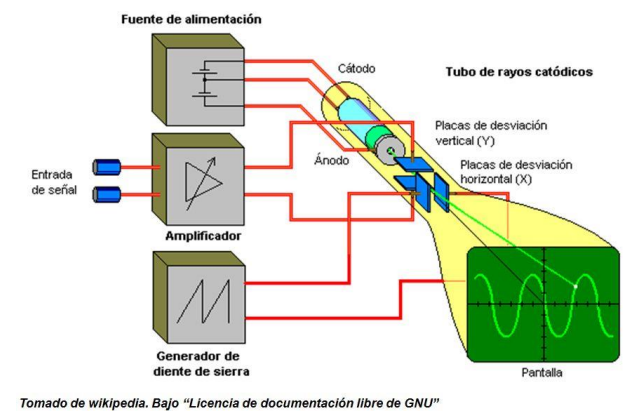
\includegraphics[width=\linewidth]{F1}
\end{center}
\caption{Tubo de rayos catódicos}
\label{F1}
\end{figure}

Entre el ánodo y la pantalla existen dos juegos de placas deflectoras,
perpendiculares entre sí. Las placas de deflexión horizontal “X” producen un campo
eléctrico uniforme, que desvía lateralmente el haz electrónico del eje del tubo. Las
placas de deflexión vertical “Y” producen el mismo efecto pero en la dirección
vertical.\par
La función de ambos juegos de placas es la de cambiar la posición del flujo luminoso
que aparece en la pantalla P, cuando los electrones chocan con la pantalla
fluorescente que la recubre.\par
La rejilla de mando R, al ser polarizada en una forma determinada, permite el paso
de un número mayor o menor de electrones, con lo que cambia la intensidad del
punto de la pantalla.
\begin{figure}[H]
\begin{center}
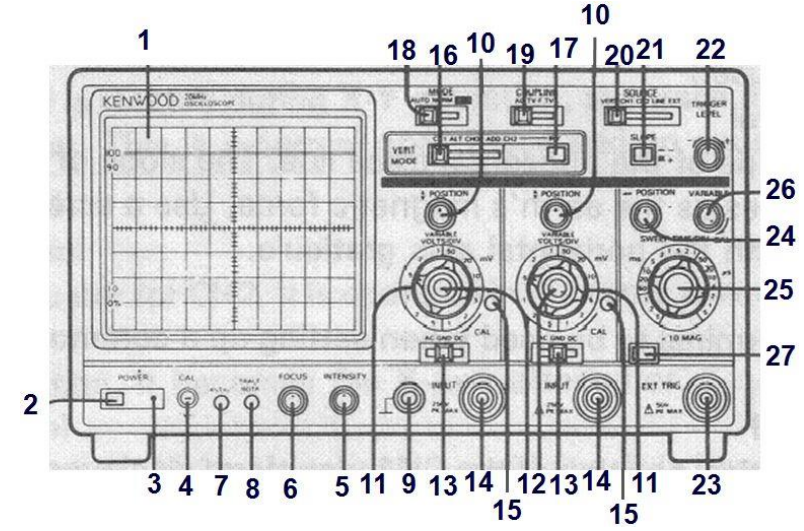
\includegraphics[width=\linewidth]{F2}
\end{center}
\caption{Osciloscopio de rayos catódicos}
\label{F2}
\end{figure}
\begin{itemize}
\item[1.] \textbf{Tubo de rayos catódicos:} La superficie efectiva de la pantalla tiene un área de 8 divisiones de 1 cm. cada una en el eje vertical y de 10 divisiones de 1 cm. cada una en el eje horizontal. Las divisiones de los ejes centrales vertical y horizontal, tienen a su vez 5 subdivisiones de 2 mm. cada una.
\item[2.] \textbf{Botón de encendido:} Al apretar este botón se enciende la fuente de poder del osciloscopio. Si se vuelve apretar nuevamente, este se apaga.
\item[3.] \textbf{Luz piloto:} Indica que el osciloscopio está encendido.
\item[4.] \textbf{Terminal de calibración:} Terminal de voltaje para efectos de calibración. Tiene un volt pico a pico, de una onda cuadrada, cuya polaridad es positiva.
\item[5.] \textbf{Intensidad:} Botón que se utiliza para ajustar el brillo en la línea de trazo.
\item[6.] \textbf{Control de foco:} Se utiliza para ajustar el enfoque y obtener una imagen clara.
\item[7.] \textbf{Control de astigmatismo:} Para el ajuste del astigmatismo del trazo. Se debe utilizar un
desatornillador para ajustar este control, en conjunto con el control de
foco, y así obtener una imagen lo más clara posible. Una vez que se ha
corregido, no es necesario hacer ajustes adicionales en uso normal.
\item[8.] \textbf{Control de rotación:} Sirve para ajustar la pendiente de línea de trazo horizontal, la cual se altera debido a influencias tales como la fuerza magnética de la Tierra. Se debe utilizar un desatornillador pequeño para ajustar horizontalmente esta línea de trazo.
\item[9.] \textbf{Terminal de tierra:} Esta Terminal se utiliza cuando se requiere una tierra común con otro equipo.
\item[10.] \textbf{Control de posición:} Para ajustar la posición vertical de la onda en la pantalla del tubo de rayos catódicos en ambos canales respectivamente. Durante la operación x-y se utiliza para ajustar la posición del eje ``y''.
\item[11.] \textbf{VOLT/DIV:} Conmutador seleccionador de sensibilidad vertical. Este conmutador puede ajustarse para que la señal mostrada tenga la amplitud apropiada sobre la pantalla del osciloscopio.
\item[12.] \textbf{Control variable:} Para un fino ajuste en la sensibilidad del eje vertical. Permite un ajuste continuo de acuerdo a los rangos de VOLT/DIV. En la posición ``CA'', la sensibilidad está calibrada al valor indicado en el conmutador VOLT/DIV.
\item[13.] \textbf{Control AC-GND-DC:} Este botón selecciona el acople de la entrada del amplificador vertical. En la posición AC el acople indica corriente alterna y es utilizado para observar solo las componentes de la señal AC. La posición DC indica corriente directa, y dicho acople permite observar todas las componentes, incluyendo la DC. En la posición GND se manda una señal del amplificador a tierra. Esta última posición permite verificar el nivel cero.
\item[14.] \textbf{Terminal de entrada:} Botón de entrada del eje vertical para el Canal 1 y el Canal 2 respectivamente. Durante la operación ``x-'', este se transforma en el botón de entrada del eje ``y''.
\item[15.] \textbf{Control de balance:} Para el ajuste del balance de la corriente directa y cada uno de los canales. Sin embargo, se pueden presentar discrepancias debido a variaciones de temperatura en la habitación. Un desatornillador pequeño ayuda al ajuste de este control, de tal manera que el trazo no se mueva de arriba a abajo cuando se hace girar el control de VOLT/DIV.
\item[16.] \textbf{Control selector de modo vertical:} Para seleccionar el modo de operación del eje vertical.
\begin{itemize}
\item \textbf{CH1:} Para hacer aparecer la señal de entrada del Canal 1 en la
pantalla.
\item \textbf{ALT:} Alterna las señales de entrada de los canales 1 y 2 para cada barrido, y los muestra en la pantalla.
\item \textbf{CHOP:} Para mostrar las señales de entrada del Canal 1 y Canal 2 en la pantalla, independientemente del barrido.
\item \textbf{ADD:} Para mostrar en la pantalla la forma de onda de ambos canales de manera combinada. Sin embargo, cuando el Canal 2 está en inverso, la diferencia entre ambos canales se muestra en la pantalla.
\item \textbf{CH2:} Para hacer aparecer la señal de entrada del Canal 2 en la
pantalla.
\end{itemize}
\item[17.] \textbf{Botón de inverso:} Cuando este botón está presionado, la señal de entrada en Canal 2 aparecerá invertida.
\item[18.] \textbf{Botón selector de modo:} Selecciona los modos de disparo.
\item[19.] \textbf{Selector de acople:} Selecciona el acople de disparo. En AC la señal de disparo es acoplada capacitivamente al circuito de disparo. La componente de corriente directa es eliminada. Se utiliza el acople AC para medidas normales de formas de onda. TV-F y TV-L se utilizan para aplicaciones especiales.
\item[20.] \textbf{Perilla seleccionadora de fuente:} Se utiliza para seleccionar la señal de disparo de la fuente.
\begin{itemize}
\item \textbf{VERT:} La señal de disparo de la fuente será seleccionada por el modo vertical.
\item \textbf{CH1:} La señal de disparo en Canal 1 será la señal de disparo.
\item \textbf{CH2:} La señal de disparo en Canal 2 será la señal de disparo.
\item \textbf{LINE:} La forma de la onda de la fuente de voltaje comercial se
convertirá en la señal de disparo.
\item \textbf{EXT:} La señal de disparo en el botón EXT-TRIG se convertirá en la
fuente de la señal de disparo.
\end{itemize}
\item[21.] \textbf{Botón de pendiente:} Para seleccionar la polaridad de la pendiente de la señal. Cuando el botón está afuera el disparo se verá con la señal aumentando, y cuando el botón está presionado, la señal se verá descendiendo.
\item[22.] \textbf{Control de nivel de disparo:} Para el ajuste del nivel de disparo. Esto determinará a que puntos de la pendiente se iniciará el barrido de la señal.
\item[23.] \textbf{Entrada para disparo externo:} Entrada para señales generadas externamente. Cuando el botón``SOURCE'' se coloca en``EXT'', la señal de entrada a través de la terminal se convertirá en la fuente de la señal de barrido.
\item[24.] \textbf{Control de posición:} Para el ajuste de la posición horizontal de la onda que aparece en la pantalla.
\item[25.] \textbf{Control SWEEP TIME/DIV:} Control del tiempo de barrido por división. Sirve para seleccionar el tiempo de barrido. Se puede seleccionar desde 0.5 \si{\micro\second}/DIV hasta 0.5 \si{\second}/DIV.
\item[26.] \textbf{Control de variable:} Un ajuste de tiempo de barrido continuo puede ser obtenido fuera del rango de SWEEP TIME/DIV. El tiempo de barrido será compensado moviendo la perilla ``cal'' a la derecha.
\item[26.] \textbf{Control multiplicador por 10:} Presione este botón para aumentar por 10 la señal de la pantalla hacia la derecha e izquierda, tomando como referencia en centro de la pantalla.
\end{itemize}
\chapter{Guía para la presentación de informes de laboratorio}
La información que se proporciona en esta Guía tiene por finalidad ayudar al
estudiante a presentar la información obtenida en los laboratorios. El formato
puede variar de acuerdo a las características particulares de la práctica que se
esté realizando. Sin embargo, se espera que se tenga en todos los casos un orden
lógico de presentación en el informe.\\
El informe de laboratorio debe realizarse utilizando LateX, basado en la respectiva plantilla que se encontrara en el TecDigital, siguiendo los lineamientos que esta proporciona.\\
El informe se recibirá únicamente en electrónico a la dirección que el profesor
designe el primer día de lecciones, de común acuerdo con los alumnos.\\
El alumno
al enviar el informe entiende y acepta que este se puede seleccionar como
muestra en el proceso de acreditación y explícitamente está de acuerdo en dar su
permiso de uso para tal fin.\\
El informe debe escribirse en forma impersonal (tercera persona) y en
pasado. Se deberá utilizar el sistema internacional de unidades.
\section{Estructura}
\begin{itemize}
\item \textbf{Portada}\\
Deberá utilizarse la portada para informes de laboratorio que se adjunta en la respectiva plantilla.
\item \textbf{Tabla de contenidos}\\
Se utilizara el sistema de autogeneracion incluido en la plantilla.
\item \textbf{Objetivos}\\
Deben indicar la finalidad del trabajo que se realizó. Estos objetivos aparecen
indicados en cada una de las prácticas a realizar.
\item \textbf{Materiales y equipo}\\
Debe incluir el listado completo del equipo utilizado para realizar el laboratorio,
esta información también está disponible en las prácticas a realizar. A pesar de lo
anterior, este apartado debe indicar los instrumentos realmente usados en la
práctica, si por algún motivo estos cambiaran.
\item \textbf{Procedimiento}\\
Corresponde a una descripción de los procedimientos empleados, la cual debe ser
lo suficientemente completa como para permitir una reproducción del trabajo. La
organización de esta sección es simple y cronológica y debe indicar la razón de
cada paso realizado.\\
Esta información también está disponible en las prácticas a realizar. A pesar de lo
anterior, este apartado debe indicar el procedimiento realmente seguido en la
práctica, si por algún motivo este cambiara
\item \textbf{Resultados teoricos y experimentales}\\
Generalmente se incluyen cuadros y gráficos que encierran un resumen de
resultados teóricos y prácticos, así como porcentajes de error entre los mismos.
Nunca se presenta una discusión o interpretación de los mismos.
No se recomienda aglomerar demasiada información en un cuadro. El título de las
tablas, cuadros o gráficos debe concordar con los datos correspondientes, e incluir
las unidades de medida cuando corresponda.
El número y nombre de la tabla o cuadro se escribe en la parte superior, como
encabezado. En la parte inferior debe aparecer un comentario corto y explicativo
que indique la fuente de los datos obtenidos. En el caso de figuras, éstas se
rotulan en la parte inferior con número y título. Debe aparecer en todos los casos
las unidades y parámetros de los ejes, así como la escala utilizada.
La numeración de los títulos debe ser auto generada por el programa Word ® o
equivalente. Toda figura, ilustración, ecuación, tabla, gráfico, cuadro, etc. debe ser
numerada y contener título.
\item \textbf{Discusion de resultados}\\
Se discuten e interpretan los resultados obtenidos con base en los objetivos
establecidos. Se indican causas y efectos, así como límites y defectos de los
resultados obtenidos. En este apartado se debe hacer referencia a los aspectos
que relacionen lo observado con lo medido, así como lo que indican los autores en
la literatura citada. Es importante que quede claramente establecido el aporte del
autor del informe en discusión.
\item \textbf{Conclusiones}\\
En esta sección se hace un listado claro y conciso de las conclusiones a las que
llega el autor del reporte, sobre los aspectos que incluye el laboratorio. Las
conclusiones se presentan como oraciones, sin explicación, ya que la esta se
encuentra en la discusión.\\
\item \textbf{Apendices}\\
Incluye una serie de aspectos importantes que el lector del informe podrá
consultar para\begin{itemize}
\item \textbf{Teoría}\\
Debe aparecer una síntesis de los fundamentos teóricos del tema, con información
actualizada, que sirva para comparar, discutir y apoyar las implicaciones
relacionadas o derivadas del trabajo hecho. Dicha revisión debe ir respaldada por
la bibliografía consultada, ya que de otra forma no es válida. No se debe copiar
información que aparezca en esta Guía de Laboratorio.\\
\item \textbf{Muestra de calculos}\\
Es un resumen de fórmulas o procedimientos utilizados para hacer los cálculos
teóricos. Deben aparecer los resultados obtenidos, pero no las operaciones que se
realizaron para llegar a ellos.
\item \textbf{Nomenclatura}\\
ndicar las abreviaturas utilizadas en el reporte y el significado que las mismas
tienen en el contexto del reporte presentado.\\
\end{itemize} 
\item \textbf{Referencias bibliográficas}\\
Todas las publicaciones contenidas en esta sección deben haber sido citadas en
el texto. Las referencias blbliograficas se realizaran bajo el formato IEEE. Por ejemplo si desea citar el ``Alexander'' lo puede hacer así: \cite{alexander2006fundamentos}. 
\end{itemize}

\chapter{Lineamientos para la presentación de la bitácora}
Como parte del trabajo a realizar por los estudiantes del curso del “Laboratorio de
Electricidad II” se requiere que presenten una bitácora técnica con sus
experiencias en el laboratorio. El objetivo de esta sección es brindar una serie de
lineamientos para la elaboración adecuada de esta bitácora.
La bitácora muestra las experiencias que tuvo la persona que realizó el
experimento de tal forma que otra persona pueda repetir este. Por lo tanto, la
bitácora debe indicar claramente los objetivos, los materiales utilizados, el equipo,
los valores de los componentes, el procedimiento, los circuitos, los valores
esperados y los obtenidos, si se cumplieron los objetivos planteados, cualquier
recomendación u opinión que sea pertinente, así como cualquier otra información
que quien la escribe considere importante.
La bitácora no es un informe técnico formal (que se detalló en la sección anterior),
por lo que tiene algunas diferencias. Entre ellas se numeran:
\begin{itemize}
\item La bitácora se llena exclusivamente a mano con bolígrafo color azul.
\item La redacción es en pasado (incluyendo los objetivos y el procedimiento), y
como es un documento que detalla la experiencia de quien realizó el
laboratorio, debe escribirse preferiblemente en primera persona.
\item No se deben dejar espacios vacíos en esta, si un espacio no corresponde
llenarlo se debe “matar el espacio”, esto se hace con una línea encima del
espacio. En caso que sean muchos espacios colindantes se puede pasar
una línea curva sobre todos ellos.
\item Todos los gráficos, tablas, ilustraciones o figuras se deben encerrar en un
cuadro.
\item Como la bitácora es una reseña de las experiencias, es recomendable que
los materiales, procedimientos, resultados, conclusiones y otros se
presenten como parte de un solo texto que explique lo encontrado, y no
como títulos por separado.
\item La bitácora se debe presentar por duplicado, en el caso de la que usa la
Escuela el papel produce la copia de una vez sin necesidad de papel
carbón. La hoja blanca (donde se escribe) es el original que le corresponde
al profesor y la verde es la copia que se deja el alumno.
\item Todas las hojas de la bitácora se deben firmar por el alumno en el espacio
“Firma Responsable”. Al recibir la bitácora el profesor firma en el espacio
“Firma Testigo”.
\item Es completamente válido presentar impresos los gráficos, tablas,
ilustraciones o figuras; sin embargo, se debe colocar la misma información
en la hoja de copia ya sea impresa o a mano.
\end{itemize}
Se debe utilizar una hoja gruesa debajo de la hoja de copia (verde) al realizar la
bitácora. Como la copia se hace automáticamente a presión si no se usa esta hoja gruesa para proteger las demás hojas estas quedarán marcadas. La bitácora
viene con una hoja índice para tal fin, en esta se debe escribir el nombre de cada
uno de los laboratorios que se encuentran en la bitácora.
La bitácora es un documento legal que refleja el trabajo realizado, debido a esto,
no se permite usar corrector u otro producto que borre el contenido (ya que
introduce dudas sobre la veracidad de la información). El estudiante debe prestar
suma atención para no tener que hacer correcciones; si debe realizar algún
cambio se traza una línea sobre la información incorrecta, firmar encima de la
corrección y colocar el nuevo dato a la par o en otra parte del documento
(debidamente referenciado dónde).
Todas las hojas de la bitácora vienen con un consecutivo, por ninguna
circunstancia este se debe perder. Consecuentemente, si por alguna razón se
debe prescindir de una hoja se debe colocar una leyenda grande a mano que diga
“NULO” o “ANULADO” y firmar la hoja.
Los campos de la bitácora se deben llenar de la siguiente forma:
\begin{enumerate}
\item \textbf{Libro No.} Si la información de las experiencias de laboratorio ocupan varias
bitácoras, estas se numeran. En caso que solo se vaya a utilizar una
bitácora este campo “se mata”.
\item \textbf{Nombre:} Del estudiante; marcar además el campo respectivo, deje los
otros dos en blanco (“Profesor” y “Otro”).
\item \textbf{Nombre del proyecto:} Nombre del curso.
\item \textbf{Número de proyecto:} Número consecutivo del laboratorio implementado.
\item \textbf{Experimento:} Nombre del laboratorio implementado.
\item \textbf{Fecha:} En que se pasó la bitácora. No se coloca la fecha en que se hizo el
laboratorio, si esta última se debe indicar se hace en el texto.
\item \textbf{Protección:} Estos campos no se usan por lo que se deben “matar”.
\item \textbf{Firma Responsable:} Del alumno al entregar la bitácora.
\item \textbf{Firma Testigo:} Del profesor al recibir.
\end{enumerate}
Por último, los laboratorios se deben reportar en el orden en que se realizaron, no
es permitido saltarlos o bien reportarlos de otra forma.

\chapter{Seguridad en laboratorios de electricidad, instructivo para el estudiante}
Cuando se trabaja con electricidad es imprescindible que se tenga claro los
riesgos que conlleva el trabajar con corriente eléctrica. Esta, aunque no es la
principal causa de accidentes, cuando ocurren son graves y en muchos casos
mortales.\\
Las consideraciones que se citan a continuación deben ser acatadas por el
estudiante cuando trabaje en los laboratorios, pero más importante aún, cuando
en su vida profesional se vea expuesto a situaciones en donde exista corriente
eléctrica.\\
\begin{itemize}
\item \textbf{Riesgo de incendio}\\
Los incendios provocados por causas eléctricas ocurren principalmente por:
\begin{itemize}
\item Sobrecarga de conductores que provoca calentamiento en cables y equipo.
\item Sobrecalentamiento debido a fallas de equipo de control
\item Fallas en el aislante de conductores.
\item Combustión de materiales inflamables por cercanía a equipos de baja
tensión (papel, madera)
\item Combustión de materiales inflamables por chispas o arcos (thinner,
pinturas, etc.)
\end{itemize}
\item \textbf{Shock electrico}\\
El shock eléctrico, dependiendo de su intensidad, puede causar desde una
sensación de cosquilleo, hasta estímulos musculares dolorosos que podrían
provocar la pérdida total del control muscular y llegar hasta la muerte.
Los mecanismos de muerte por electricidad son:
\begin{itemize}
\item Fibrilación ventricular. Se denomina fibrilación ventricular al trastorno del
ritmo cardiaco que presenta un ritmo ventricular rápido (>250 latidos por
minuto), irregular, de morfología caótica y que lleva irremediablemente a la
pérdida total de la contracción cardiaca, con una falta total del bombeo
sanguíneo y por tanto a la muerte del paciente.
\item Tetanización. Es un proceso por el cual un músculo deja de responder a los
estímulos que lo hacen contraer voluntariamente y por lo tanto moverse,
demostrando que estamos vivos y respiramos. Se manifiesta por la
contracción de los músculos de las extremidades, lo que trae como
consecuencia que la víctima quede prendida al conductor.
\item Doble acción. Tetanización y fibrilación a la vez
\item Parálisis bulbar. Afecta predominantemente de los nervios que controlan la
masticación, la deglución y el habla.
\item Parálisis cardio circulatoria y respiratoria.
\end{itemize}
\item \textbf{Factores a considerar para evitar accidentes}\\
\begin{enumerate}
\item \textbf{Intensidad de la corriente}
\begin{itemize}
\item En corriente alterna, el umbral mínimo de percepción es 1,1 mA.
\item El umbral mínimo de contracción muscular ocurre con 9 mA,
pudiendo ocurrir contracción de los músculos, que expele al
accidentado lejos del conductor. De no ser así, se podría llegar a la
asfixia por contracción de los músculos respiratorios.
\item En corriente alterna el umbral de corriente peligroso corresponde a
80 mA, donde se puede llegar a fibrilación ventricular.
\item Entre 3 o 4 amperios de corriente puede llegar a causar depresión
del sistema nervioso central
\end{itemize}
Esto se puede resumir de la siguiente manera:
\begin{table}[H]
	\caption{Prueba del corto circuito.}
	\label{tab:ACT1}
	\centering
	\begin{tabular}[t]{| >{\centering\arraybackslash}m{2cm} | >{\arraybackslash}m{8cm} |}
		\hline
		\textbf{Intensidad} & \textbf{Posible efecto en el cuerpo} \\
		\hline
		De 2 a 4 mA & Temblor de los nervios en los dedos hasta el antebrazo. \\
		\hline
		De 5 a 7 mA & Leve sensación de choque, no doloroso aunque incómodo.
		La persona promedio puede soltar la fuente que proporciona
		corriente. Reacciones involuntarias al choque pueden
		resultar en lesiones \\
		\hline
		De 10 a 15 mA & Sensación desagradable, pero todavía es posible soltarse \\
		\hline
		De 19 a 22 mA & Fuertes dolores de brazo. Ya no es posible soltarse
		voluntariamente. \\
		\hline
		De 25 a 50 mA mA & Irregularidades cardiacas, aumento de presión arterial,
		efecto de tetanización, inconsciencia y fibrilación ventricular. \\
		\hline
		De 50 a 200 mA mA & Menos de medio ciclo cardiaco: No se da fibrilación.
		Fuerte contracción muscular.
		Menos de un ciclo cardiaco: Fibrilación, inconsistencia.
		Marcas visibles. Paro cardiaco reversible.
		Más de un ciclo cardiaco: Quemaduras \\
		\hline
		Mayor a 4 A & Parálisis cardiaca y respiratoria. Quemaduras graves. Con
		toda probabilidad, puede causar la muerte. \\
		\hline
		10 A & Paro cardiaco, quemaduras severas y con toda probabilidad,
		puede causar la muerte. \\
		\hline
		\end{tabular}
\end{table}
\item \textbf{Resistencia eléctrica del cuerpo}
Esta depende de muchos factores, por lo que es difícil de determinar. El elemento
principal en la resistencia del cuerpo humano es la resistencia de la piel, la cual
varía de persona a persona. Esta disminuye si se está enfermo, se tienen lesiones
en la piel y si el ambiente circundante es húmedo.\\
La resistencia entre 2 partes opuestas del cuerpo puede estar en el orden de los
kilo ohmios, aunque puede ser de apenas unas decenas de ohmios entre partes
cercanas, sobre todo si la piel está humedecida.\\
Bajo condiciones secas la piel humana es muy resistente. Si la piel está húmeda,
la resistencia del cuerpo baja considerablemente.
\begin{itemize}
\item Condiciones secas: $I=\frac{V}{R}=\frac{120 V}{100000 \Omega}=1,2 \ mA$\\
\item Condiciones húmedas: $I=\frac{V}{R}=\frac{120 V}{1000 \Omega}=120 \ mA$\\
\item La intensidad de la corriente (amperes) es el factor fundamental para poder
predecir el tipo de daño que la electricidad puede causar al cuerpo.
\item Voltajes menores a 20 o 30 voltios son inofensivos excepto en ciertos lugares muy
sensibles del cuerpo tales como la boca, labios, lengua, genitales, etc. Por encima
de esos voltajes, la corriente que circula puede llegar a provocar daños graves e
incluso la muerte.
\end{itemize}
\item \textbf{Factores en que cuenta el tiempo de contacto}\\
Para que se produzca fibrilación en el corazón se requiere que el contacto sea de
al menos del orden de un período cardiaco medio, que es del orden de 0,75 s.
Tiempos de contacto menores a eso no producen fibrilación.\\
Esto es muy importante desde el punto de vista de la protección que suministran
los disyuntores diferenciales, ya que el corte de corriente en ellos se produce en
tiempos aproximados de 200 milisegundos, a efecto de que el organismo no sea
atravesado por corrientes peligrosas.
\item \textbf{Formas de corriente}\\
\begin{itemize}
\item Tanto en corriente alterna como en continua se aplica la Ley de
Ohm.
\item La corriente continua puede producir electrólisis pero teniendo en
cuenta el tiempo de exposición y la tensión
\item La corriente alterna, en igualdad de condiciones, es de 3 a 4 veces
menos peligrosa que la corriente continua.
\item No obstante, en términos generales, 100 mA, tanto la corriente
continua como la alterna, son peligrosamente mortales.
\end{itemize}
\item \textbf{Otras consideraciones}\\
\begin{itemize}
\item La susceptibilidad es mayor si la persona está haciendo un buen
contacto con tierra, tal como cuando está apoyada a superficies
húmedas o majadas.
\item Ambientes con alta temperatura, en donde la transpiración de las
personas se incrementa, presentan un riesgo adicional, porque el
aislamiento que proporciona la ropa se ve reducida debido a la
humedad.
Se pueden producir quemaduras al pasar corriente eléctrica por el
cuerpo, en especial en los puntos de contacto con los conductores
eléctricos.
\item Descargas eléctricas tales como chispas o arcos, pueden encender
vapores inflamables, causando explosiones y fuego.
\item En el laboratorio, el shock eléctrico es posible que sea leve, pero
puede generar otros riesgos por la reacción refleja de sobresalto,
que puede hacer que el afectado o sus compañeros pierdan el
control de materiales y equipo que se esté manipulando, causando
otro tipo de accidentes.
\end{itemize}
\end{enumerate}
\end{itemize}

\chapter{Normas de seguridad en el laboratorio}

\begin{itemize}
\item \textbf{Hábitos de conducta}\\
\begin{itemize}
\item No fumar en los laboratorios por seguridad e higiene.
\item No consumir alimentos ni bebidas dentro del laboratorio.
\end{itemize}

\item \textbf{Mantener el puesto de trabajo limpio}\\
\begin{itemize}
\item La mesa de trabajo debe estar libre de abrigos, bolsos, libros, etc.
\item No dejar bultos u otros objetos en los lugares de circulación, en especial
entre los pupitres.
\end{itemize}

\item \textbf{Salud}\\
\begin{itemize}
\item Si tiene algún padecimiento, o si se usa algún medicamento que
considere relevante para el curso normal de la práctica, esta debe
informarse al profesor antes de realizar la práctica.
\item No ingresar al laboratorio bajo los efectos de drogas o alcohol.
\end{itemize}

\item \textbf{Vestimenta}\\
\begin{itemize}
\item En trabajos con máquinas o en sus inmediaciones, no se debe vestir
con prendas sueltas o con partes que cuelguen, como por ejemplo,
corbatas, flecos, etc.
\item No se deben usar sandalias, zapatos abiertos o tacón alto en el
laboratorio.
\item Usar camisas de manga larga de algodón. Materiales sintéticos pueden
provocar que en un accidente de quemadura esta se adhiera a la piel.
Se sugiere el uso de gabacha, que no sea larga ni floja, de algodón o
con un porcentaje alto de este
\item Usar pantalón largo.
\item No se debe, al realizar la práctica, llevar anillos, relojes de pulsera,
collares u otros accesorios que puedan engancharse, tales como
“piercings” en cualquier parte del cuerpo.
\item En caso de que se tenga pelo largo, se debe llevar recogido con el fin de
evitar riesgos.
\item Realizar los laboratorios con ropa seca y en superficies secas.
\end{itemize}

\item \textbf{En general}\\
\begin{itemize}
\item En los laboratorios no se deben gastar bromas, ni jugar, ni comunicarse
con gritos.
\item Estudiar atentamente la guía del laboratorio a realizar.
\item Seguir en todo momento las instrucciones del profesor. Ante cualquier
duda, consultar al profesor.
En prácticas de laboratorio supervisadas, no se debe energizar ningún
panel o fuente de voltaje sin que el profesor haya revisado la instalación
correspondiente.
\item No se pueden realizar experimentos que no estén autorizados por el
profesor.
\item Mantener el debido respeto hacia el profesor, los compañeros y
compañeras.
\item No utilizar el celular durante las sesiones de laboratorio. Mantenerlo
apagado.
\end{itemize}

\item \textbf{Equipo de proteccion}\\
De manera particular, y según sea la naturaleza del laboratorio, será indispensable
utilizar equipo de protección.
Esto será indicado por el profesor en cada laboratorio en particular, teniendo en
consideración los riesgos que tenga el mismo.
Esto incluye:
\begin{itemize}
\item Uso de anteojos o pantallas de protección en operaciones donde exista
riesgo de salpicadura.
\item Uso de guantes aislantes o protectores cuando se trabaja con piezas
cortantes
\item Uso de cascos, mascarillas y calzado especial cuando estos se
requieran.
\end{itemize}
\item \textbf{Maquinas}\\
En algunas ocasiones no se puede eliminar el riesgo en el origen y por tanto es
necesario utilizar medios de protección colectiva, tales como resguardos o
dispositivos de seguridad.
El resguardo es un componente de una máquina que se utiliza como barrera
material para garantizar la protección.
Un dispositivo de protección es aquel que impide que se inicie o se mantenga una
fase peligrosa de la máquina, mientras se detecta o sea posible la presencia
humana en la zona de peligro.\\
Por tanto:
\begin{itemize}
\item No ponga fuera de servicio los dispositivos de seguridad existentes.
\item Utilice correctamente los elementos de seguridad.
\item No utilice equipos y maquinaria sin conocer su funcionamiento.
\item Antes de realizar cualquier tarea en una máquina, siga atentamente
las instrucciones. En caso de duda, pregunte al profesor(as).
Desconectar de la red eléctrica las herramientas y equipos antes de
proceder al ajuste.
\item No reparar, desatascar o limpiar equipo. Notificar la anomalía para
que el personal capacitado realice la tarea.
\item No bloquear sistemas electrónicos, eléctricos, mecánicos, etc.
\end{itemize}
\end{itemize}


%----------------------------------------------------------------------------------------
%	BIBLIOGRAPHY
%----------------------------------------------------------------------------------------

\bibliographystyle{ieeetr}

\bibliography{manual}

%----------------------------------------------------------------------------------------


\end{document}